\documentclass[11pt]{article}

\usepackage{graphicx}

\usepackage{array}

\usepackage{xcolor}

\usepackage[a4paper,total={8in,10in}]{geometry}

\usepackage{mdframed}

\usepackage{mdwlist}

\usepackage{geometry}

\usepackage{marginnote}

\usepackage{multicol}

\usepackage{hyperref}


\begin{document}
\textit{Contact-9910988199}                                                 \hspace{2.5cm}\textit{E-mail: divyansh.sgs@gmail.com}\hspace{2.5cm}\textit{LinkedIn: http://bit.ly/2p2MgXg}                           
\begin{mdframed}[backgroundcolor=orange]

~

\begin{flushright}

\begin{Huge}

\color{white}{\fontfamily{pbk}\selectfont Divyansh}\color{gray}{\fontfamily{pbk}\selectfont\textbf{Malhotra}}

\end{Huge}

\end{flushright}
\end{mdframed}

\textit{Address: Flat -135, Sec-12, Pkt-2, Dwarka, New Delhi-110075}\hspace{2.5cm}\textit{Electronics and Communication Engineer}
\begin{figure}[ht]
\begin{minipage}[b]{0.45\linewidth}
\centering
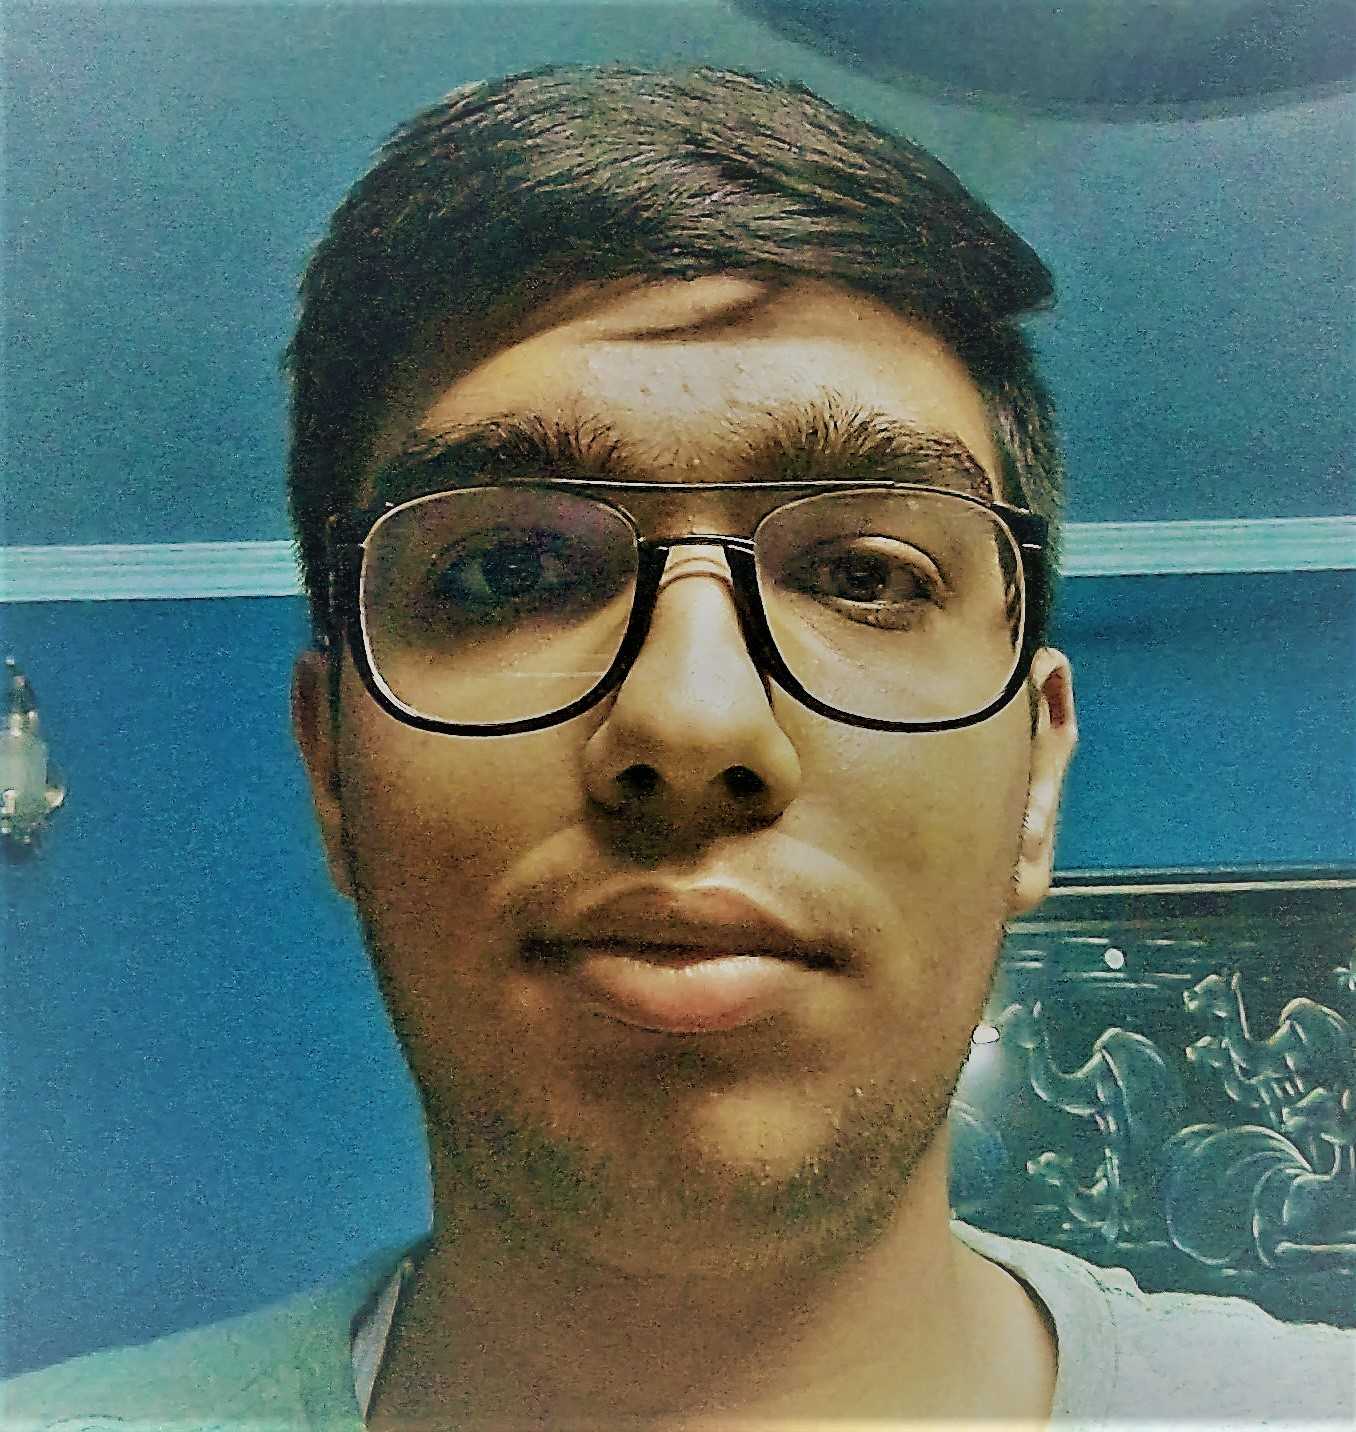
\includegraphics[scale=0.095]{photo.jpg}
\end{minipage}
\hspace{0.5cm}
\begin{minipage}[b]{0.45\linewidth}
\flushleft
I am an enthusiastic, imaginative and a full of energy student. I am a person who is open to all ideas, who hears all, analyses the data and then makes his own decisions. My nickname, as anointed by one of my professors, is the compiler because I tend to find the errors and work towards correcting them, not only in codes but also in life. I put my heart and soul into the work that I take up and am always eager to learn new skills everyday so that today, I can outshine my yesterday.

\end{minipage}
\end{figure}
\end{document}